\documentclass[12pt]{article}
\usepackage{xcolor}
\usepackage{booktabs}
\usepackage{csquotes}
\usepackage{langsci-gb4e}
\usepackage{hyperref}
\hypersetup{
    colorlinks=true,
    linkcolor=blue,
    filecolor=magenta,
    citecolor=blue,      
    urlcolor=cyan,
    pdftitle={whose-gorilla},
    pdfpagemode=FullScreen,
}
\usepackage[style=langsci-unified,backend=biber]{biblatex}
\addbibresource{refs.bib}
\usepackage{amsmath}
\usepackage{amssymb}
\usepackage{tcolorbox}
\usepackage{tikz}
\usepackage{microtype}
\usepackage{float}
\usetikzlibrary{arrows.meta,shapes,positioning}
\usepackage{orcidlink}

% Define only used colors
\definecolor{lsLightBlue}{RGB}{201,233,246}
\definecolor{lsDOIGray}{RGB}{0,0,0}

% Define upright subscripts
\newcommand{\listener}{\mathrm{L}}

\title{Grammaticality de-idealized\\[4pt]
       \large Lingbuzz preprint v0.2 – 15 June 2025\\[6pt]
       \normalsize \url{https://github.com/brettr/gdi}}
\author{Brett Reynolds \orcidlink{0000-0003-0073-7195}\\Humber Polytechnic \& University of Toronto
\thanks{I used ChatGPT o3-pro and Claude Opus 4 in drafting this version of the paper.\\This work is licensed under CC-BY 4.0}}
\date{}

\begin{document}
\maketitle

\begin{abstract}
\small
Speakers reject *\textit{I've finished it yesterday} (aspect semantics clash) yet accept the semantically odd \textit{Colorless green ideas sleep furiously} (no morphosyntactic clash). They block *\textit{Which did you buy car?} categorically, while linguists judge the unreadable centre‑embedding \textit{The rat the cat the dog chased killed ate the cheese} "grammatical".  
The Morphosyntactic–Meaning Model of Grammaticality (MMMG) explains such contrasts by treating grammaticality as the stability of community‑specific form–meaning pairings, not as autonomous syntax or raw frequency.

Six interacting components decide an utterance's status:  
(1) conventional morphosyntactic--meaning pairings;  
(2) compatibility between those meanings and lexical, discourse, pragmatic, and indexical meaning;  
(3) incremental‑processing limits;  
(4) socio‑pragmatic indexicality;  
(5) degree of community entrenchment;  
(6) categorical structural bans.

MMMG separates objective grammaticality \(G(u)\) from the subjective feeling of error \(F(u)\), showing why processing overload can make grammatical sentences feel wrong and why compelling semantics can mask true violations.  
A simple formalisation models entrenchment as logistic growth derived from utterance-selection dynamics, predicting S‑curves in language change. The framework yields falsifiable claims about which violations satiate under exposure, how morphosyntactic integration conditions cross‑linguistic variation, and why L2 learners over‑detect errors.  
Grounding grammaticality in community conventions while acknowledging universal processing constraints, MMMG unifies phenomena that elude purely formal or purely usage‑based accounts.
\end{abstract}

\section{Executive overview}

\paragraph*{Claim.}%
Grammaticality is the \emph{community stability} of morphosyntactic form–meaning pairings.

\paragraph*{Mechanism.}%
Six interacting constraints—pairings, semantic fit, processing load, indexicality, entrenchment, and structural bans—combine to yield an objective score \(G(u)\) and a subjective score \(F(u)\).

\paragraph*{Why this matters.}%
The configuration predicts which violations satiate, why some rare patterns remain grammatical, and how gradient “illusions” arise without abandoning categorical structure.

\bigskip
The constraints determining grammatical stability are:

\begin{enumerate}
\item \textbf{Pairings} – conventional links between morphosyntax and meaning
\item \textbf{Semantic fit} – alignment between the meaning encoded by the morphosyntax (features, argument structure, information‐status) and the semantic types and discourse roles contributed by the lexical items
\item \textbf{Processing load} – limits of incremental parsing
\item \textbf{Indexicality} – social meanings the form must carry
\item \textbf{Entrenchment} – degree of community acceptance
\item \textbf{Structural bans} – configurations blocked outright
\end{enumerate}

These constraints explain why
\begin{itemize}
    \item \textit{I've finished it yesterday} fails (semantic clash),  
    \item centre embeddings \emph{feel} wrong (processing overload) yet remain licit, and
    \item left‑branch extractions like \textit{Which did you buy car?} never improve with exposure (structural ban).
\end{itemize}
Objective grammaticality \(G(u)\) and the subjective feeling of error \(F(u)\) can therefore diverge.


\section{Motivation: The impasse in grammaticality theory}

Three long‑standing tensions block a unified account of (un)grammaticality.

\subsection{Categorical rules vs gradient judgements}

\textcite{chomsky1957} cast grammaticality as an all‑or‑nothing property.  
The competence–performance split was meant to park gradience in a separate "performance" box, yet doing so lets supportive data count as grammar and contrary data count as noise \parencite[71]{schutze2016}.

\ea
\textit{The bread the baker the apprentice helped made is delicious.}
\z
Centre‑embedded relatives are routinely labelled "grammatical but unprocessable," which merely restates the puzzle: speakers feel them to be wrong.

\subsection{Form vs meaning}

The famous \textit{Colorless green ideas sleep furiously} shows syntactic well‑formedness without plausibility.  The converse also matters:

\ea[*]{\textit{I've finished it yesterday.}}\z
Here the present‑perfect feature [+current relevance] clashes with the adverb's [+completed past], and speakers reject the sentence.  Construction‑grammar work \parencite{goldberg1995constructions} confirms that morphosyntactic meaning and lexical meaning must cohere, explaining why \textit{She texted him the address} passes while \textit{*She disappeared him the evidence} does not.

\subsection{Universal principles vs community conventions}

Labovian sociolinguistics \parencite{labov1972} shows that grammaticality is community‑relative.  Languages differ not just in lexicon but in which form–meaning pairings are conventionalised.  Usage‑based models capture frequency effects, yet they still face cases where extremely rare patterns remain grammatical and frequent patterns are blocked.

\medskip
These three tensions—categorical vs gradient, form vs meaning, universal vs communal—underline the need for a framework that explains why particular patterns of acceptability recur across speakers and across languages.


\section{Six components of (un)grammaticality}

Grammaticality, on this view, is the community stability of a form–meaning pairing; six forces determine that stability:


\subsection{Morphosyntactic form–meaning pairings within communities}

\begin{tcolorbox}[colback=lsLightBlue!30]
\textbf{Diagnostic}: Does the morphosyntactic form evoke a conventionalised meaning in this community?

\textbf{Example}: \textit{*Can the have running?}~— no viable form–meaning pairing.

\textbf{Counter‑example}: \textit{Colorless green ideas sleep furiously}~— odd semantics, but the form maps transparently to a compositional meaning.
\end{tcolorbox}

At root, grammaticality depends on stable pairings between morphosyntactic forms and meanings that a speech community has conventionalised. Forms are inherently meaningful: the English past tense usually marks past time but can index social distance (\textit{Could you?}) or low likelihood (\textit{If I went …}).

Communities define their own pairings:
\ea
\textit{Estábamos lifting en el gym.} (Spanish–English bilingual)\\
`We were lifting in the gym.'
\z
This is grammatical in communities that accept code‑mixed progressives, but ungrammatical for monolingual Spanish speakers, who expect \textit{levantando pesas} `lifting weights'.

\subsection{Semantic fit}

\begin{tcolorbox}[colback=lsLightBlue!30]
\textbf{Diagnostic}: Do the morphosyntactic meaning and the lexical/discourse meaning align?

\textbf{Example}: \textit{*I've finished it yesterday}~— present‑perfect 'current relevance' clashes with \textit{yesterday}'s 'completed past'.

\textbf{Counter‑example}: \textit{I've just finished it}~— perfect combines smoothly with \textit{just}.
\end{tcolorbox}

Even when the syntax is well‑formed, a construction fails if meanings conflict:
\ea[*]{\textit{I have 25 years.} \hfill (intended: `I'm 25 years old')}
\z
In English, \textit{have + years} denotes relational predication (e.g. experience), not age ascription.

\subsection{Processing load}

\begin{tcolorbox}[colback=lsLightBlue!30]
\textbf{Diagnostic}: Can the sentence be incrementally parsed within memory limits?

\textbf{Example}: \textit{The rat the cat the dog chased killed ate the cheese}~— multiple embeddings overwhelm processing.

\textbf{Counter‑example}: \textit{The rat that the cat killed ate the cheese}~— single embedding remains processable.
\end{tcolorbox}

Multiple centre‑embeddings overload working memory even though the structure is, in principle, grammatical \autocite{gibson2000}.

\subsection{Socio‑pragmatic indexicality}

\begin{tcolorbox}[colback=lsLightBlue!30]
\textbf{Diagnostic}: Does the form index the intended social stance or identity?

\textbf{Example}: \textit{vos} forms in a strict‑\textit{tú} region~— indexical mis‑fit.

\textbf{Counter‑example}: \textit{vos} in Buenos Aires~— indexically appropriate.
\end{tcolorbox}

\ea
¿\textit{Vos querés un café?} (Río de la Plata Spanish)\\
`Do you want a coffee?'
\z
The choice of \textit{vos} indexes regional identity; speakers outside the region may reject it for indexical reasons even though the syntax is fine.

\subsection{Community entrenchment}

\begin{tcolorbox}[colback=lsLightBlue!30]
\textbf{Diagnostic}: Is the pairing conventional within the community?

\textbf{Example}: \textit{*We counted three sheeps}~— regular plural blocked by entrenched irregular.

\textbf{Counter‑example}: \textit{We bought three computer mouses}~— recent regularisation already accepted.
\end{tcolorbox}

Transparent patterns can fail if they lack communal backing.  The independent relative \textit{whose} is so rare that many speakers never conventionalise it:
\ea[\textsuperscript{?}]{\textit{I saw Joan, a friend of whose was visiting.}}
\z

\subsection{Structural bans}

\begin{tcolorbox}[colback=lsLightBlue!30]
\textbf{Diagnostic}: Does the sentence violate a categorically blocked configuration?

\textbf{Example}: \textit{*\hspace{0.2ex}Which\hspace{0.2ex} did you buy \_ car?} — determiner extraction.

\textbf{Counter‑example}: \textit{Which car did you buy \_?} — the whole NP is extracted.
\end{tcolorbox}

Some configurations are universally rejected regardless of meaning, processing, or frequency.  They never improve with familiarity and show categorical unacceptability. While we treat these as yielding $\mu(u)=\varnothing$, an alternative is to model them as extreme biases in an utterance-selection framework—an empirically testable distinction.


\section{Quick‑diagnosis decision tree}

The six components can be queried in sequence to classify an utterance on first pass. The tree locates the first component whose failure suffices to render an utterance ungrammatical; later nodes are not evaluated once a zero value is returned.

\begin{figure}[H]
\centering
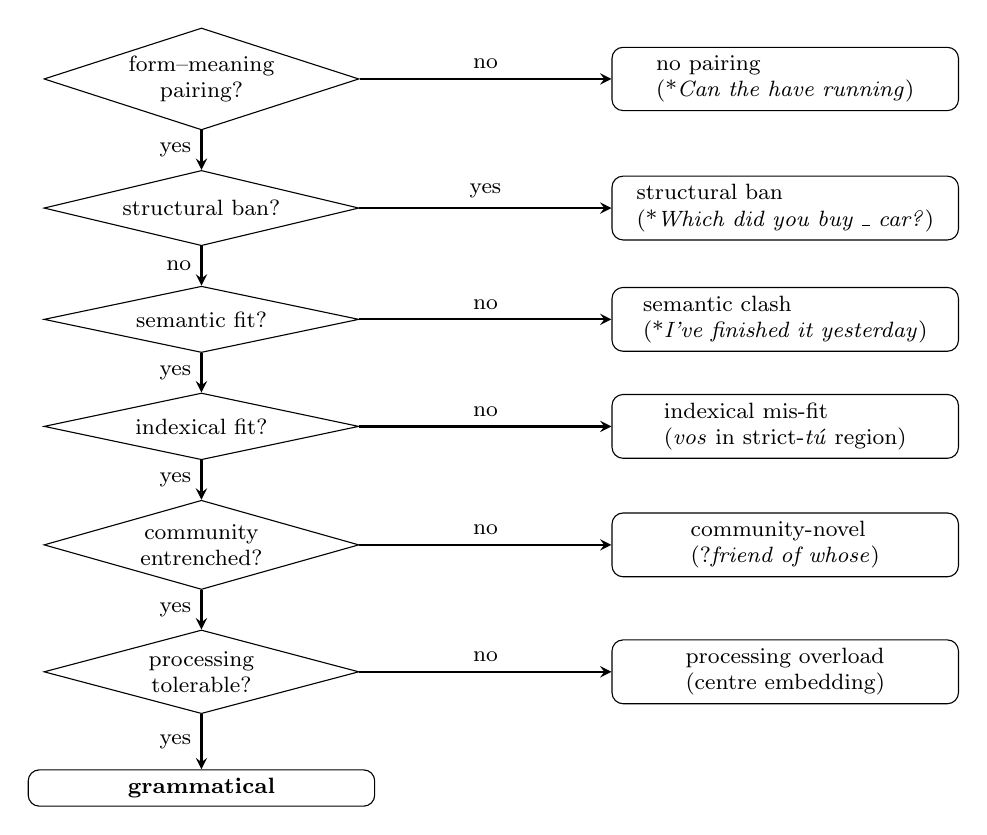
\begin{tikzpicture}[
  font=\footnotesize,                       % smaller text everywhere
  node distance = 0.5cm and 3.2cm,         % tighter vertical gap
  decision/.style = {diamond,
                     aspect=3,              % width : height = 3 : 1  →  flatter
                     draw,
                     align=center,
                     minimum width=4cm,
                     inner sep=1pt},
  outcome/.style  = {rectangle,
                     draw,
                     rounded corners,
                     align=left,
                     minimum width=4.4cm,
                     inner sep=3pt},
  arrow/.style    = {->, >=stealth, thick}
]

\node[decision] (map)  {form–meaning\\pairing?};
\node[outcome , right=of map]  (nonsense) {no pairing\\(*\textit{Can the have running})};

\node[decision, below=of map]  (ban)  {structural ban?};
\node[outcome , right=of ban]  (lbe)  {structural ban\\(*\textit{Which did you buy \_ car?})};

\node[decision, below=of ban]  (sem)  {semantic fit?};
\node[outcome , right=of sem]  (clash) {semantic clash\\(*\textit{I've finished it yesterday})};

\node[decision, below=of sem]  (idx)  {indexical fit?};
\node[outcome , right=of idx]  (misfit) {indexical mis‑fit\\(\textit{vos} in strict‑\textit{tú}~region)};

\node[decision, below=of idx]  (ent)  {community\\entrenched?};
\node[outcome , right=of ent]  (novel) {community‑novel\\(?\textit{friend of whose})};

\node[decision, below=of ent]  (proc) {processing\\tolerable?};
\node[outcome , right=of proc] (over) {processing overload\\(centre embedding)};

\node[outcome , below=0.7cm of proc] (gram) {\textbf{grammatical}};

\draw[arrow] (map)  -- node[above] {no} (nonsense);
\draw[arrow] (map)  -- node[left]  {yes} (ban);
\draw[arrow] (ban)  -- node[above] {yes} (lbe);
\draw[arrow] (ban)  -- node[left]  {no}  (sem);
\draw[arrow] (sem)  -- node[above] {no}  (clash);
\draw[arrow] (sem)  -- node[left]  {yes} (idx);
\draw[arrow] (idx)  -- node[above] {no}  (misfit);
\draw[arrow] (idx)  -- node[left]  {yes} (ent);
\draw[arrow] (ent)  -- node[above] {no}  (novel);
\draw[arrow] (ent)  -- node[left]  {yes} (proc);
\draw[arrow] (proc) -- node[above] {no}  (over);
\draw[arrow] (proc) -- node[left]  {yes} (gram);

\end{tikzpicture}
\caption{Decision tree for first‑pass diagnosis; variable names match Table~\ref{tab:notation}}
\end{figure}


The tree is a heuristic: it points to the first component that fails.  
The underlying grammar is \(G(u)=C^{t} \cdot K(u)\); when any factor is zero, the utterance is objectively ungrammatical even if later nodes would succeed.

\section{Notation}

\begin{table}[htbp]
\centering
\small
\caption{Symbols used in the formal model. Type abbreviations: struc.\ = syntactic structure, fea.\ = feature bundle, indic.\ = observed indicator}
\label{tab:notation}
\begin{tabular}{@{}llp{7cm}@{}}
\toprule
Symbol & Type & Meaning / construction method \\ 
\midrule
\multicolumn{3}{@{}l}{\textit{Utterance-level observables}} \\
$u$ & token & Concrete utterance under evaluation \\
$M(u)$ & struc. & Morphosyntactic parse of $u$ \\
$\mu(u)$ & fea. & Morphosyntactic meaning unpacked from $M(u)$ \\
$\sigma(u)$ & fea. & Composite lexical–pragmatic meaning intended \\[0.5em]
\multicolumn{3}{@{}l}{\textit{Evaluation scores}} \\
$K(u)\in[0,1]$ & score & Semantic compatibility of $\mu(u)$ with $\sigma(u)$ \\
$G(u)\in[0,1]$ & score & Objective grammaticality; product defined in Eq.~\eqref{eq:G} \\
$F(u)\in[-1,0]$ & score & Listener's felt ill‑formedness; see Eq.~\eqref{eq:F} \\[0.5em]
\multicolumn{3}{@{}l}{\textit{Community latent variable and indicators}} \\
$C^{t}(u)\in[0,1]$ & latent & Community entrenchment at time $t$ \\
$A(u)$ & indic. & Availability in memory (recognition hit rate) \\
$E(u)$ & indic. & Exposure frequency (log corpus count) \\
$P(u)$ & indic. & Production probability (elicitation rate) \\
$S(u)$ & indic. & Social acceptability (matched-guise score) \\[0.5em]
\multicolumn{3}{@{}l}{\textit{Parameters and drift components}} \\
$\lambda_{\listener}$ & param & Listener weight on objective violation, Eq.~\eqref{eq:F} \\
$\gamma$ & param & Processing‑to‑affect scaling, Eq.~\eqref{eq:F} \\
$\eta$ & noise & Listener-specific bias term \\
$\Delta(u)$ & drift & Net entrenchment bias, Eq.~\eqref{eq:delta} \\
$\alpha_{\mathrm{sem}}$ & param & Weight on semantic transparency \\
$\alpha_{\mathrm{soc}}$ & param & Weight on social prestige \\
$\alpha_{\mathrm{struct}}$ & param & Weight on structural analogy \\
$\beta_{\mathrm{noise}}$ & param & Noise penalty coefficient \\
$\beta_{\mathrm{hi}}$, $\beta_{\mathrm{lo}}$ & const & High/low noise penalty values \\
\multicolumn{3}{@{}l}{\textit{Diagnostic predictors}} \\
$\text{Transp}(u)$ & measure & Semantic transparency (role-entropy) \\
$\text{Prest}(u)$ & measure & Social prestige of innovators (7-point scale) \\
$\text{Analo}(u)$ & measure & Structural analogy pressure \\
\multicolumn{3}{@{}l}{\textit{Processing functions}} \\
$\text{ProcessingCost}(u)$ & z-score & Integration cost following \textcite{gibson2000} \\
$\text{IC}(w_i)$ & count & Integration cost at word $w_i$ \\
\bottomrule
\end{tabular}
\end{table}

\newpage
\section{Minimal formal skeleton}

\subsection{Core architecture}

The model treats grammaticality as emerging from the interaction of morphosyntactic structure, meaning compatibility, and community conventions. Figure~\ref{fig:causal-dag} shows the causal dependencies using Structural Causal Model semantics \parencite{pearl2009}.

\begin{figure}[htbp]
\centering
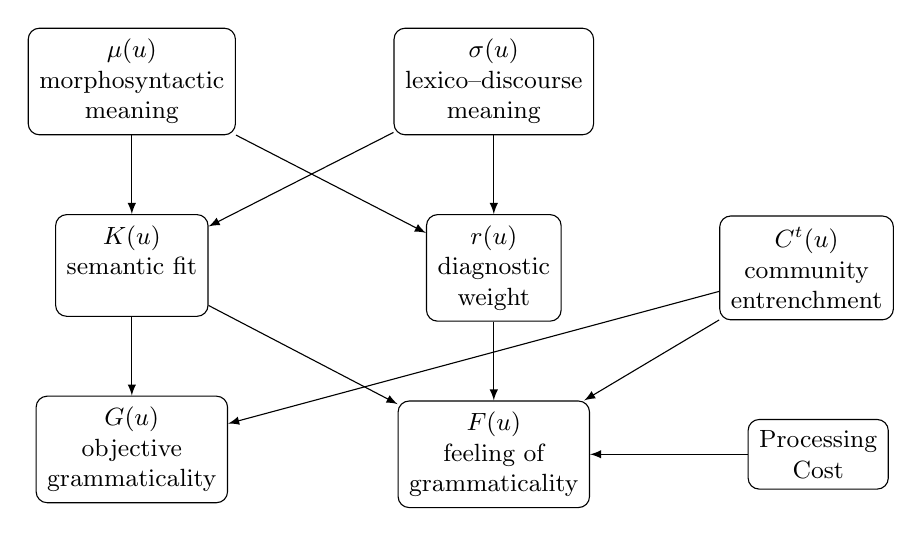
\begin{tikzpicture}[
  node distance = 1cm and 2.0cm,
  > = latex,
  var/.style = {rectangle, draw, rounded corners, align=center,
                inner sep=4pt, font=\small}
]
% ───────── 1st row ─────────
\node[var] (mu)    {$\mu(u)$\\morphosyntactic\\meaning};
\node[var, right=of mu] (sigma) {$\sigma(u)$\\lexico–discourse\\meaning};

% ───────── 2nd row ─────────
\node[var, below=of mu]     (K) {$K(u)$\\semantic fit\\};
\node[var, below=of sigma]  (r) {$r(u)$\\diagnostic\\weight};

% ───────── 3rd row ─────────
\node[var, right=of r] (C) {$C^{t}(u)$\\community\\entrenchment};

% ───────── 4th row ─────────
\node[var, below=of K]      (G) {$G(u)$\\objective\\grammaticality};
\node[var, below=of r]      (F) {$F(u)$\\feeling of\\grammaticality};

% ───────── exogenous ───────
\node[var, right=of F] (P) {Processing\\Cost};

% ───────── arrows ──────────
\draw[->] (mu)    -- (K);
\draw[->] (sigma) -- (K);
\draw[->] (mu)    -- (r);
\draw[->] (sigma) -- (r);

\draw[->] (K) -- (G);
\draw[->] (C) -- (G);

\draw[->] (K) -- (F);
\draw[->] (r) -- (F);
\draw[->] (C) -- (F);
\draw[->] (P) -- (F);
\end{tikzpicture}
\caption[Macro-level causal structure]%
{\textbf{Macro-level causal structure of the MMMG.} All arrows encode Structural Causal Model semantics; e.g., $\text{do}(C^{t} \leftarrow 0) \Rightarrow G = 0$ by definition of $G = C^{t}K$. Since $P$ has no parents except exogenous noise, there is no open back-door into $F$ once $K$ and $r$ are conditioned on.
\\\emph{Input layer}: the parser maps the surface form to a morphosyntactic meaning $\mu(u)$
and the discourse context supplies a lexico–discourse meaning $\sigma(u)$, which include indexical meanings.
Any categorical structural ban makes this mapping fail, i.e.\ $\mu(u)=\varnothing$.
\\\emph{Fit layer}: the compatibility score $K(u)\!\in[0,1]$ already folds together ordinary
semantic fit, indexical coherence, and the hard zero caused by a mapping failure.
The diagnostic weight $r(u)$ is the cue-based probability that the parser detects the
violation. 
\\\emph{Community layer}: speech-community entrenchment $C^{t}(u)$ multiplies with the
compatibility score to yield objective grammaticality,
$G(u)=C^{t}(u)K(u)$.
\\\emph{Output layer}: felt ill-formedness is
$F(u)= -\lambda_{\mathrm L}\,r(u)\!\bigl(1-K(u)\bigr)
       -\gamma\,\text{ProcessingCost}(u)+\eta$,
where ProcessingCost is computed via integration cost. $F(u)\!\in[-1,0]$, where 0 means `no negative signal'.
\\\emph{Heuristic mapping}: pairings $\to\mu(u)$;
semantic fit \& indexicality $\to\sigma(u),K(u)$;
structural bans $\to\mu(u)=\varnothing$;
processing load $\to$ ProcessingCost and $r(u)$;
entrenchment $\to C^{t}(u)$.}
\label{fig:causal-dag}
\end{figure}

\subsection{Grammaticality function}

For an utterance $u$, objective grammaticality is:
\begin{equation}\label{eq:G}
G(u)=C^{t}(u)\cdot K(u)
\end{equation}
where $K(u) = 0$ whenever the form–meaning mapping fails.

\subsection{Subjective feeling function}

The listener's subjective feeling of (un)grammaticality is:
\begin{equation}\label{eq:F}
F(u)= -\lambda_{\listener}\,(1-G(u)) \;-\; \gamma\,\text{ProcessingCost}(u) + \eta
\end{equation}
where:
\begin{itemize}
  \item $\lambda_{\listener} \in [0,1]$ — listener-specific penalty weight for objective violations
  \item $\gamma > 0$ — conversion factor mapping processing load to negative affect
  \item $\text{ProcessingCost}(u) = \sum_{i} \text{IC}(w_i)$ — sum of integration costs following \textcite{gibson2000}
  \item $\eta \sim \mathcal{N}(0,\sigma^{2})$ — idiosyncratic listener bias
\end{itemize}

$F(u)$ is constrained to $[-1,0]$: 0 means `no negative signal'; larger negative values indicate stronger perceived ill-formedness.

The processing cost operationalizes memory load via dependency integration:
\begin{equation}
\text{IC}(w_i) = \sum_{d \in \text{deps}(w_i)} |d|
\end{equation}
where $|d|$ is the linear distance in intervening discourse referents. This aligns with established psycholinguistic metrics \parencite{futrell2020}, allowing direct comparison with reading-time data.

\subsection{Worked example}

Consider $u=$\,*\textit{I've finished it yesterday}:

\begin{itemize}
  \item Form–meaning mapping succeeds: present‑perfect morphology evokes 'current relevance'
  \item $K(u)=0$ because that meaning clashes with \textit{yesterday} ('completed past')
  \item $C^{t}(u)=1$ since the construction is fully entrenched in English
  \item Therefore $G(u)=1\times0=0$ (objectively ungrammatical)
\end{itemize}

With illustrative values $\lambda_{\listener}=0.8$, $\gamma=0.1$, $\text{ProcessingCost}(u)=0.2$, $\eta=0$:
\begin{equation}
F(u)=-0.8(1-0)-0.1\cdot0.2=-0.82
\end{equation}
yielding a strong negative feeling.

\subsection{Community entrenchment as latent variable}

To avoid circularity, $C^{t}(u)$ is treated as a latent cause of four observables:\footnote{The latent variable $C^{t}$ is identifiable up to scale given monotone relationships with at least three indicators and appropriate factor-loading constraints.}
\begin{equation}
C^{t}(u)\ \longrightarrow\ 
\begin{cases}
A(u) & \text{availability in memory}\\
E(u) & \text{exposure frequency}\\
P(u) & \text{production probability}\\
S(u) & \text{social acceptability}
\end{cases}
\end{equation}
Each indicator follows a measurement model with error:
\begin{equation}
\log E(u) = \lambda_E C^{t}(u) + \epsilon_E, \quad \epsilon_E \sim \mathcal{N}(0,\sigma_E^{2})
\end{equation}
and similarly for the other indicators. This specification allows for measurement uncertainty while maintaining identifiability.

Each indicator is collected with different methodology:
\begin{itemize}
  \item \textbf{Availability} $A(u)$: recognition hit rates or lexical-decision latencies
  \item \textbf{Exposure} $E(u)$: log token counts in balanced corpora
  \item \textbf{Production} $P(u)$: proportion in sentence-completion tasks
  \item \textbf{Social acceptability} $S(u)$: matched-guise appropriateness scores
\end{itemize}

The latent variable $C^{t}(u)$ is estimated via confirmatory factor analysis without re-using acceptability data.

\subsection{Community dynamics}

\begin{figure}[h]
\centering
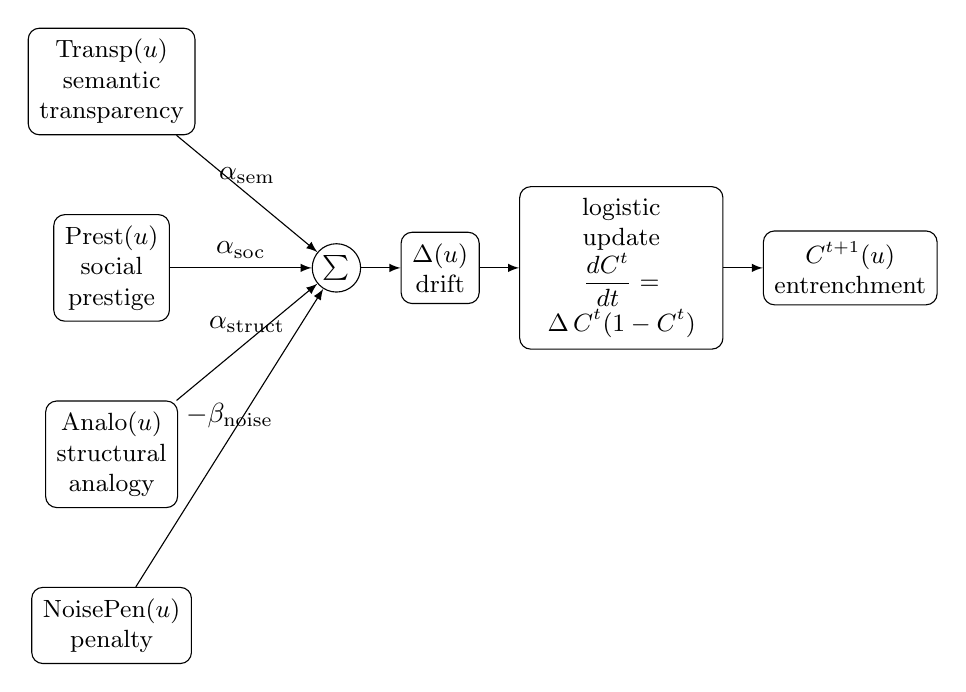
\begin{tikzpicture}[
  node distance = 1cm and 0.5cm,
  > = latex,
  var/.style = {rectangle, draw, rounded corners,
                align=center, inner sep=4pt, font=\small},
  sum/.style = {circle, draw, inner sep=1.5pt, font=\small}
]
% inputs
\node[var] (transp) {Transp$(u)$\\semantic\\transparency};
\node[var, below=of transp] (prest) {Prest$(u)$\\social\\prestige};
\node[var, below=of prest] (analo) {Analo$(u)$\\structural\\analogy};
\node[var, below=of analo] (noise) {NoisePen$(u)$\\penalty};

% weighted sum
\node[sum, right=1.8cm of prest] (sum) {$\sum$};

% arrow labels with weights
\draw[->] (transp) -- node[above] {$\alpha_{\mathrm{sem}}$} (sum);
\draw[->] (prest)  -- node[above] {$\alpha_{\mathrm{soc}}$} (sum);
\draw[->] (analo)  -- node[above] {$\alpha_{\mathrm{struct}}$} (sum);
\draw[->] (noise)  -- node[above] {$-\beta_{\mathrm{noise}}$} (sum);

% delta node
\node[var, right=of sum] (delta) {$\Delta(u)$\\drift};

% logistic integrator
\node[var, right=of delta] (logi) {\parbox{2.3cm}{\centering logistic\\update\\$\displaystyle\frac{dC^t}{dt}=\! \Delta\,C^t(1-C^t)$}};

% entrenchment
\node[var, right=of logi] (C) {$C^{t+1}(u)$\\entrenchment};

% arrows
\draw[->] (sum)   -- (delta);
\draw[->] (delta) -- (logi);
\draw[->] (logi)  -- (C);
\end{tikzpicture}
\caption{Community‑entrenchment update pathway.\label{fig:entrenchment-circuit}}
\end{figure}


Change in entrenchment follows logistic growth, derived from mean-field approximation of utterance-selection dynamics \parencite{blythe2012}:
\begin{equation}
\frac{dC^{t}(u)}{dt}= \Delta(u)\,C^{t}(u)\bigl(1-C^{t}(u)\bigr)
\end{equation}

As given in Eq.~\eqref{eq:delta}, the net drift bias is:
\begin{equation}\label{eq:delta}
\Delta(u)=
   \alpha_{\mathrm{sem}}\!\cdot\!\text{Transp}(u)+
   \alpha_{\mathrm{soc}}\!\cdot\!\text{Prest}(u)+
   \alpha_{\mathrm{struct}}\!\cdot\!\text{Analo}(u)-
   \beta_{\mathrm{noise}}\cdot\text{NoisePen}(u)
\end{equation}

Components:
\begin{itemize}
    \item $\text{NoisePen}(u)$: Binary penalty if surprisal $> \theta$ and self-repair rate $> \theta'$
    \item $\text{Transp}(u)$: Semantic transparency (lower role-entropy = more transparent)
    \item $\text{Prest}(u)$: Social prestige of innovating group (7-point scale)
    \item $\text{Analo}(u)$: Structural analogy pressure from related patterns
    \item $\alpha_{\mathrm{sem/soc/struct}} \sim \mathcal{N}(\mu_\alpha, \tau_\alpha^2)$: Hierarchically pooled weights
\end{itemize}

The hierarchical specification $\alpha_j \sim \mathcal{N}(\mu_\alpha, \tau_\alpha^2)$ with weakly informative priors on $\tau_\alpha$ prevents overfitting while allowing community-specific variation.


\section{Predictions and Falsifiability}

\subsection{S-Curve Dynamics}

The logistic equation predicts:
\begin{itemize}
\item \textbf{If} $\Delta(u) > 0$ \textbf{then} construction shows increasing entrenchment following S-curve \textbf{(available data)}
\item \textbf{If} $\Delta(u) < 0$ \textbf{then} construction remains marginal or decreases in acceptability \textbf{(available data)}
\item \textbf{If} $\Delta(u) \approx 0$ \textbf{then} heightened variability and sensitivity to external factors \textbf{(planned study)}
\end{itemize}

\subsection{L2 Trajectory}

L2 learners should show:
\begin{itemize}
\item \textbf{Initial stage}: Input appears as noise lacking meaningful structure \textbf{(planned ERP study)}
\item \textbf{Intermediate stage}: Heightened sensitivity, marking many native patterns as ungrammatical \textbf{(available data)}
\item \textbf{Advanced stage}: Gradual alignment with community norms \textbf{(available data)}
\end{itemize}

\subsection{Cross-Linguistic Gender Test}

Pronoun-antecedent gender mismatches should trigger:
\begin{itemize}
\item \textbf{Spanish}: Strong ungrammaticality (gender permeates morphosyntax) \textbf{(planned experiment)}
\item \textbf{English}: Moderate ungrammaticality (gender limited to pronouns) \textbf{(available data)}
\item \textbf{Japanese}: Pragmatic infelicity only (no grammatical gender) \textbf{(planned experiment)}
\end{itemize}

\subsection{Satiation Scope}

Repeated exposure should increase acceptability for:
\begin{itemize}
\item Low-frequency constructions (independent relative \textit{whose}) \textbf{(planned experiment)}
\item Processing-difficult patterns (reduced relatives) \textbf{(available data)}
\item Semantic mismatches (novel metaphors) \textbf{(available data)}
\end{itemize}

But NOT for:
\begin{itemize}
\item Categorical violations (determiner extraction) \textbf{(available data)}
\item Fundamental mapping failures (word salad) \textbf{(available data)}
\end{itemize}

\subsection{Comparison with Noisy-Channel Accounts}

The MMMG makes distinct predictions from noisy-channel models \parencite{gibson2013} for grammatical illusions. While both predict mismatches between intuition and structure, MMMG additionally predicts:
\begin{itemize}
\item Community-specific illusion strengths based on entrenchment differences
\item Systematic variation in which constructions show satiation effects
\item Quantitative differences in acceptability decline rates (measurable via $\Delta \text{AIC}$)
\end{itemize}

\section{Positioning Relative to Existing Theories}

\begin{table}[h]
\centering
\small
\caption{Coverage of key issues across frameworks (✓ = explicit/integrated, ∼ = partial, ✗ = absent)}
\begin{tabular}{@{}lcccc@{}}
\toprule
Framework & Form–meaning & Gradience & Community & Processing \\
          & integration  & handled   & variation & effects \\
\midrule
Early Generative     & $\sim$ & $\times$ & $\sim$ & $\times$ \\
GB/Minimalism        & $\sim$ & $\sim$   & $\sim$ & $\times$ \\
Construction Grammar & $\checkmark$ & $\sim$ & $\sim$ & $\sim$ \\
Usage-Based          & $\checkmark$ & $\checkmark$ & $\checkmark$ & $\sim$ \\
MMMG (this work)     & $\checkmark$ & $\checkmark$ & $\checkmark$ & $\checkmark$ \\
\bottomrule
\end{tabular}
\end{table}


\subsection{Key distinctions}

\textbf{Versus generative grammar} —  
MMMG retains the insight that certain configurations are systematically excluded, but explains these "structural bans" as the outcome of extreme, community‑level stability rather than as inviolable innate rules.

\textbf{Versus Construction Grammar} —  
Both frameworks treat constructions as form–meaning pairings, yet MMMG gives special status to \emph{morphosyntactic} pairings: violations in this layer trigger qualitatively stronger ungrammaticality judgments than purely pragmatic or lexical mismatches.

\textbf{Versus usage‑based models} —  
MMMG builds in frequency effects, but also accounts for systematic gaps such as the independent relative \textit{whose}: a pattern can be blocked even when its components are frequent and compositionally transparent.

\textbf{Versus relevance‑theoretic accounts} —  
Both reject an innate, autonomous syntax, yet MMMG attributes constraints to conventionalised form–meaning pairings inside a speech community, rather than to general principles of interpretive efficiency alone.


\section{Roadmap for Spin-off Papers}

\begin{table}[htbp]
\centering
\small
\caption{Planned publication sequence}
\begin{tabular}{@{}llll@{}}
\toprule
Phase & Paper & Target venue & Timeline \\
\midrule
A & Lingbuzz preprint & Repository & Month 1 \\
& Conference proceedings & LSA/GLOW & Month 6 \\
B & Manifesto article & \textit{Language}/\textit{Glossa} & Month 9 \\
C & Formal model & \textit{NLLT}/\textit{J Lang Model} & Year 2 \\
D1 & Diachronic S-curves & \textit{Lang Var Change} & Year 2-3 \\
D2 & Cross-linguistic gender & \textit{Cognitive Linguistics} & Year 2-3 \\
E & Monograph & LangSci Press & Year 3-4 \\
\bottomrule
\end{tabular}
\end{table}

Each paper can stand alone while building toward the comprehensive monograph treatment.

\section{Conclusion}

This framework reconceptualizes grammaticality as emerging from stable form-meaning pairings within language communities. The six components~-- morphosyntactic pairings, semantic compatibility, processing constraints, indexicality, entrenchment, and categorical blocking~-- interact to produce the full range of grammaticality phenomena.

The approach integrates insights from multiple traditions while making specific, falsifiable predictions. It explains both why some patterns remain stubbornly ungrammatical despite transparency and why others shift from marginal to accepted. By distinguishing objective grammaticality from subjective feelings, it accounts for mismatches between intuition and linguistic reality.

Future work should test the cross-linguistic predictions, develop computational implementations of the formal model, and explore applications to language change, acquisition, and clinical linguistics. The framework provides a foundation for understanding how human communities create and maintain the systematic form-meaning relationships we call grammar. The current model assumes well-mixed interaction patterns; structured-network extensions following \textcite{baxter2006} remain for future investigation.

\newpage
\appendix

\section{Formal Derivations}

\subsection{Measurement Model for Community Entrenchment}

The latent variable $C^t(u)$ is estimated through confirmatory factor analysis:

\[
\begin{pmatrix}
A(u) \\
\log E(u) \\
P(u) \\
S(u)
\end{pmatrix}
=
\begin{pmatrix}
\lambda_A \\
\lambda_E \\
\lambda_P \\
\lambda_S
\end{pmatrix}
C^t(u) +
\begin{pmatrix}
\epsilon_A \\
\epsilon_E \\
\epsilon_P \\
\epsilon_S
\end{pmatrix}
\]
where factor loadings $\lambda_i$ and error terms $\epsilon_i$ are estimated from data. Identifiability is achieved by fixing $\lambda_A = 1$ and constraining all loadings to be positive.

\subsection{Noise Detection Mechanism}

The relationship between exposure and entrenchment:
\[
\frac{dC^t}{dt} = f(E(u)) - \text{NoisePenalty}(u)
\]
where:
\[
\text{NoisePenalty}(u) = \begin{cases}
\beta_{\mathrm{hi}} & \text{if } \text{Surprisal}(u) > \theta_1 \text{ AND } \text{RepairRate}(u) > \theta_2 \\
\beta_{\mathrm{lo}} & \text{otherwise}
\end{cases}
\]

\subsection{Bifurcation Analysis}

Actuation occurs when $\Delta(u) = 0$. Near this critical point:
\[
C^t \approx C^* + A e^{\lambda t}
\]
where $\lambda = \Delta'(u^*) \cdot C^*(1-C^*)$ determines growth rate post-bifurcation.

\subsection{Processing Cost Function}

\begin{figure}[h]
\centering
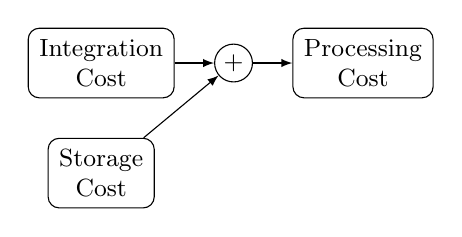
\begin{tikzpicture}[
  node distance = 0.5cm and 0.5cm,
  > = latex,
  var/.style = {rectangle, draw, rounded corners,
                align=center, inner sep=4pt, font=\small},
  sum/.style = {circle, draw, inner sep=1.5pt, font=\small}
]
\node[var] (integ) {Integration\\Cost};
\node[var, below=of integ] (stor) {Storage\\Cost};

\node[sum, right=of integ] (plus) {$+$};
\node[var, right=of plus] (P) {Processing\\Cost};

\draw[->] (integ) -- (plus);
\draw[->] (stor)  -- (plus);
\draw[->] (plus)  -- (P);
\end{tikzpicture}
\caption{Computation of the processing‑cost term.\label{fig:proc-cost}}
\end{figure}

Following \textcite{gibson2000}, Dependency Locality Theory:
\[
\text{ProcessingCost}(u) = \sum_{i} \text{IC}(w_i)
\]
where the integration cost at each word is:
\[
\text{IC}(w_i) = \sum_{d \in \text{deps}(w_i)} |d|
\]
with $|d|$ counting intervening discourse referents.

\section{Turkish Harmony Case Study}

Turkish distinguishes lexical disharmony (tolerated) from allomorphic harmony violations (ungrammatical).

\subsection{Stem-Internal: Phonology Only}

\ea
\textit{doktor} `doctor' (disharmonic stem, grammatical)
\z
No morphosyntactic feature unrealized, so $G(u) = 1$ despite phonological markedness.

\subsection{Suffixal: Morphosyntactic Requirement}

\ea
\ea[]{\textit{kitap-lar} `books' (harmonic, grammatical)}
\ex[*]{\textit{kitap-ler} (intended `books', harmony violation)}
\z
\z
The suffix must copy [±back] from stem. Wrong vowel leaves feature unrealized:
\begin{itemize}
\item Mapping succeeds (plural selected)
\item $K(u) = 0$ (feature not realized)
\item $C^t(u) = 1$ (everyone knows plural)
\end{itemize}

Therefore $G(u) = 0$, categorically ungrammatical.

\subsection{Theoretical Implications}

Turkish harmony shows morphosyntax-phonology interface effects on grammaticality. Only violations preventing feature realization trigger ungrammaticality; pure phonological dispreference affects only subjective feeling $F(u)$.

 \newpage
\begin{sloppypar}
\printbibliography[title=References]
\end{sloppypar}

\end{document}